%%%%%%%%%%%%%%%%%%%%%%%%%%%%%%%%%%%%%%%%%%%%%%%%%%%%%%%%%%%%%%%%%%%%%%%%%%%%%%%%
%2345678901234567890123456789012345678901234567890123456789012345678901234567890
%        1         2         3         4         5         6         7         8

\documentclass[letterpaper, 10 pt, conference]{ieeeconf}  % Comment this line out
                                                          % if you need a4paper
%\documentclass[a4paper, 10pt, conference]{ieeeconf}      % Use this line for a4
                                                          % paper

\IEEEoverridecommandlockouts                              % This command is only
                                                          % needed if you want to
                                                          % use the \thanks command
\overrideIEEEmargins
% See the \addtolength command later in the file to balance the column lengths
% on the last page of the document



% The following packages can be found on http:\\www.ctan.org
\usepackage{graphicx} 
\usepackage{algpseudocode,algorithm}
\usepackage{bm}
\usepackage{color}
\usepackage{subfig}
\usepackage{url}
\usepackage{floatrow}
\usepackage{amsmath}
\DeclareMathOperator*{\argmax}{arg\,max}
\DeclareMathOperator*{\argmin}{arg\,min}
\usepackage[super]{nth}

\title{\LARGE \bf
A Reinforcement Learning Approach 
for Rebalancing Vehicles in Autonomous Mobility-on-Demand Systems
}

%\author{ \parbox{3 in}{\centering Huibert Kwakernaak*
%         \thanks{*Use the $\backslash$thanks command to put information here}\\
%         Faculty of Electrical Engineering, Mathematics and Computer Science\\
%         University of Twente\\
%         7500 AE Enschede, The Netherlands\\
%         {\tt\small h.kwakernaak@autsubmit.com}}
%         \hspace*{ 0.5 in}
%         \parbox{3 in}{ \centering Pradeep Misra**
%         \thanks{**The footnote marks may be inserted manually}\\
%        Department of Electrical Engineering \\
%         Wright State University\\
%         Dayton, OH 45435, USA\\
%         {\tt\small pmisra@cs.wright.edu}}
%}

\author{Vivian Wong% <-this % stops a space
\thanks{Vivian Wong is with the Department of Civil and Environmental Engineering, Stanford University, Stanford, CA, 94305:
        {\tt\small vwwong3@stanford.edu}}%
}


\begin{document}



\maketitle
\thispagestyle{empty}
\pagestyle{empty}


%%%%%%%%%%%%%%%%%%%%%%%%%%%%%%%%%%%%%%%%%%%%%%%%%%%%%%%%%%%%%%%%%%%%%%%%%%%%%%%%
\begin{abstract}

This paper presents an approach to rebalance vehicles in Autonomous Mobility-on-Demand systems (AMoD) through a learning and a rebalancing stage. In the learning stage, we use reinforcement learning on historical data to approximate the values of each autonomous vehicle's actions. Then in the rebalancing stage, we use these values to find advantageous rebalancing actions in real-time for each available vehicle. We test this approach on real customer data from Didi Chuxing: we show that the computational complexity of this approach does not increase with the number of stations in the system, however, sacrificing 10 times of performance compared with a reactive real-time rebalancing strategy.  

\end{abstract}


%%%%%%%%%%%%%%%%%%%%%%%%%%%%%%%%%%%%%%%%%%%%%%%%%%%%%%%%%%%%%%%%%%%%%%%%%%%%%%%%
\section{Introduction}

As our cities grow rapidly everyday, transportation becomes a challenge for many urban dwellers. Among many future mobility systems, mobility-on-demand (MoD) is deemed one of the most promising modes of transportation. Together, MoD and autonomous vehicles form the mobility system of Autonomous Mobility-on-Demand (AMoD), where passengers drive vehicles to destinations, and vehicles autonomously rebalance, or disperse into the system to address future demands. Rebalancing therefore becomes crucial in AMoD in order to avoid unwanted concentration of idling vehicles in popular drop-off locations. 

\subsection{Literature}
A large amount of research has been produced in using optimization techniques to find optimal rebalancing strategies of MoD systems. However, to the best of our knowledge, all of the existing rebalancing strategies using optimization suffer from the problem of scalability. \cite{Zhang.ea:Reactive} approaches the problem by formulating it as an linear integer optimization problem, thereby rebalancing vehicles with a reactive real-time policy. \cite{Iglesias.ea:MPC} develops a model predictive control (MPC) algorithm that shows promising results, while incorporating demand forecasts into its input. However, \cite{Zhang.ea:Reactive} and \cite{Iglesias.ea:MPC} both face the problem of computational complexity growing with the size of the system. The problem size of \cite{Zhang.ea:Reactive} is an increasing function of the number of stations, or nodes, in the MoD system. On the other hand, the problem size of \cite{Iglesias.ea:MPC} is an increasing function of both the number of stations and the length of the planning horizon.
\cite{Tsao.ea:Stochastic} tackles the problem of scalability as it presents a controller that outperforms \cite{Iglesias.ea:MPC} using a stochastic MPC algorithm that incorporated demand uncertainty. The best-performing variant of the algorithm sacrificed some performance to be more scalable, making its problem size an increasing function of the number of samples in its Sample Average Approximations method, which reduces complexity, but still, could face a large problem size depending on the scenario. 

There has also been work addressing rebalancing or similar problems using reinforcement learning. \cite{Rahili.ea:Caltech},\cite{Gueriau.ea:Decentralized},\cite{Wen.ea:SharedMoDRL} and \cite{Lin.ea:DidiFleetManagement} implemented RL in an end-to-end fashion to solve problems that closely resemble vehicle rebalancing. Although each incorporated different modeling assumptions and RL algorithms, their problem size scales with fleet size. Furthermore, these approaches only provide their vehicles local information concerning the vehicles themselves. This assumption shrinks the state-space of the RL problem significantly, but cannot take in the advantage of having a fully autonomous system.

In order to optimize matches between driver and customer order in a ride-hailing service, \cite{Xu.ea:DidiDispatch} introduced an algorithm that involves 1) an offline learning step that uses historical data and reinforcement learning to estimate expected value of a driver in a state and store those values in a look up table, and 2) an online planning step that takes the value functions, and uses optimization algorithm (KM algorithm) to find best matches. However, \cite{Xu.ea:DidiDispatch} also only provide each vehicle with local information. This paper extends upon \cite{Xu.ea:DidiDispatch}'s idea, learning values from historical data in order to make rebalancing a more computationally feasible problem, while providing each vehicles both global and local information of the system, so that they can make more informed decisions.

\subsection{Motivation of proposed work} 
Due to the above-mentioned limitations in existing work, to the best of our knowledge, there is no existing approach to rebalance vehicles that 1) achieves scalability so that the computational complexity of rebalancing will not grow as a function of number of stations and vehicles, and 2) provides each vehicle with global information. This paper therefore proposes an approach to tackle these challenges.  

\subsection{Statement of work} 
The contributions of this paper are threefold. First, we develop an approach to model the problem as a Markov-Decision Process (MDP) and divide the problem into two sub-problems: a learning stage and a rebalancing stage. Second, we propose an algorithm to solve each sub-problem. In the learning stage, our algorithm aims to accurately produce estimates of state-action values through learning on historical data. In the rebalancing stage, our algorithm leverages the learned values to rebalance vehicles in real-time. Third, we validate the approach by performing an experiment using a dataset of Didi Chuxing, while comparing with the performance of the controller in \cite{Zhang.ea:Reactive} on the same dataset. Our approach shows a significant decrease in performance, but a reduction in computational complexity. 

\begin{figure}[thpb]
      \centering
      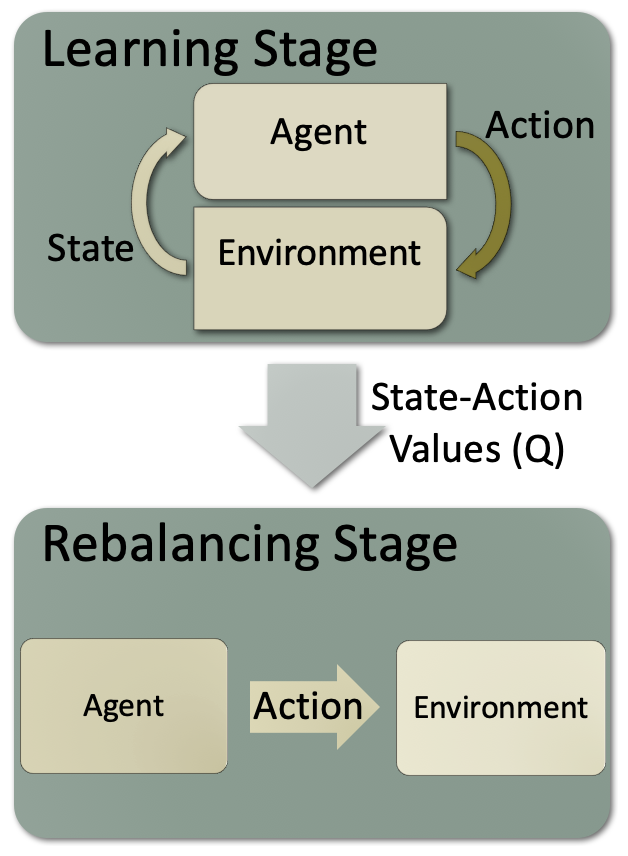
\includegraphics[scale=0.7]{procedure.png}
      \caption{Illustration of the proposed approach.}
      \label{figurelabel}
\end{figure}

%%%%%%%%%%%%%%%%%%%%%%%%%%%%%%%%%%%%%%%%%%%%%%%%%%%%%%%%%%%%%%%%%%%%%%%%%%%%%%%%
\section{Problem formulation}
\subsection{Background Information}
Consider an environment discretized into a set of $\mathcal{N}$ stations (also can be viewed as discretized regions, as in [1]). Time is presented in discrete intervals of unit time $1$. The furthest time that will be considered is denoted as $T$.

Furthermore, let $M$ denote the total number of vehicles. Let $v^e_i$ denote the difference between the number of vehicles at or arriving at station $i$, and the number of passengers preparing to board an available vehicle at station $i$, as stated in \cite{Zhang.ea:Reactive}. Note that we assume that the vehicles arrive deterministically, or that no uncertainty is taken into account for travel times between two stations. 

%%%%%%%%%%%%%%%%%%%%%%%%%%%%%%%%%%%%%%%%%%%%%%%%%%%%%%%%%%
\subsection{MDP Model Description}
At every time step $t \in \{1,...,T-1,T\}$, a MDP, an \textit{agent} observes the environment and store the values of interest in the observation as its \textit{current state, $s_t$}. The agent then conducts an \textit{action $a_t$} following a certain policy, $\pi(s_t)$. At the end of this time step (or the beginning of time step $t+1$), a \textit{new state $s_{t+1}$} and a \textit{reward $r_t$} are observed. The definitions of MDP components are:\\

\noindent \textit{Agent}: Each vehicle is treated as an agent. Although this definition makes the problem a multiagent problem, it reduces the dimensions of actions, so that there is a smaller action space to explore. \\

\noindent \textit{State, $s_t$}: The state at time step $t$ is defined as a vector of length $2|N|$, concatenated with two $|N|$ dimensional vectors, $v^e$ and $o^m$. $v^e$ stores all elements of $v^e_i$. The vector $o^m$ is the one-hot vector with value 1 at where vehicle $m$'s current station is.[TO DO: DEFINE FINAL STATE DEFINITION] \\

\noindent \textit{Action, $a_t$}: An agent is only made to choose an action when it is idle. Consider an idle agent currently at station $i$. Its action is defined as $j$, where $j\in \mathcal{N}$. If $i = j$, then the agent remains idle at its current station. If $i \neq j$, the agent departs to go to station $j$. The dimension of the action space is therefore $\mathcal{N}$. \\

\noindent \textit{Reward, $r_t$}: The reward is equal to the reduction in average customer wait time at time $t$, compared to that at time $t-1$. \\ 

Lastly, from classical MDP definitions, we define the state-action value, $Q(s,a)$ as the expected utility if following an action $a$ from state $t$.

%%%%%%%%%%%%%%%%%%%%%%%%%%%%%%%%%%%%%%%%%%%%%
\subsection{Problem Formulation}
\subsubsection{Learning Stage}
The goal in the learning stage is to output accurate estimation of the state-action values, $Q(s,a)$ for any state-action pair $(s,a)$.

For state $s_t$ and action $a_t$ at time $t$, we define the predicted state-action values, $Q(s_t,a_t;\textbf{w})$ as the ${a_t}^{th}$ row of $\textbf{w}x_t$,
where $\textbf{w}$ is the weight matrix, and $x_t$ is the state vector $s_t$ plus a term accounting for bias. 

At each time step, we use new information in this time step to improve our prediction. The objective of the learning stage can therefore be formally written as:

\begin{equation}
    \min J = [Q(s_t,a_t;\textbf{w}) - (r_t+\gamma  Q(s_{t+1},a_{t+1};\textbf{w}))]^2
\end{equation}
where $\gamma$ is the future reward discount factor, which is adjustable parameter.\\

%%%%%%%%%%%%%%%%%%%%%%%%%%%%%%%%%%%%%%%%%%%%%%%%%%%%%%%%%

\subsubsection{Rebalancing Stage}
Actions that give highest state-action values for each agent may be only optimal locally but not globally. At this stage, we aim to use the state-action values learned in the learning stage to find actions that maximize the sum of values of all cars. 

The objective of this stage is that for every time step $t$
\begin{equation}
        \min -\sum_m^M Q^m(s_t,a_t;\textbf{w})\forall i,j\in \mathcal{N}
\end{equation}
where $Q^m(s_t,a_t;\textbf{w})$ is the state-action value corresponding to vehicle $m$ taking action $a_t$ under state $s_t$. 

\section{Proposed Solution}
\subsection{Learning Stage}
Due to the large size of the state-space, we will use the SARSA with value-function approximation (VFA) algorithm to approximate the state-action values. Each vehicle at each time step is a data point that the algorithm use to update the weight matrix. The algorithm is as follows:
\begin{algorithm}[H]
\caption{Learning Stage: SARSA with VFA}
\begin{algorithmic}
\For{each ($s_t,a_t,r_t,s_{t+1},a_{t+1}$)}
    \State $Q_{target} = r_t+\gamma  Q(s_{t+1},a_{t+1})$
    \State  $Q_{prediction} = Q(s_t,a_t)$
    \State J = $(Q_{prediction} - Q_{target})^2$
    \State $\textbf{w} \leftarrow \textbf{w} - \alpha \nabla_{ \textbf{w}} J$
\EndFor
\end{algorithmic}
\end{algorithm}

In this algorithm, we parameterize state-action values as a function of state, action and a weight matrix, in order to predict the values for unseen states as well. The algorithm approaches convergence as the objective in (1) is met.

\subsection{Rebalancing Stage}
In the rebalancing stage, we find the global optimum by assigning actions probabilistically for each vehicle. The algorithm follows: 
\begin{algorithm}[H]
\caption{Rebalancing Stage: Probabilistically Performing Actions}
\begin{algorithmic}
\For{each time step $t \in {0,1,...,T}$}
    \For{each vehicle $m$}
        \If {vehicle is idle}
            \State $P_j = \frac{Q(s_t,j)}{\sum_a Q(s_t,a)}$
            \State $a_t^m \leftarrow j$ with probability $P_j$
        \EndIf
    \EndFor
    \State\textbf{Assign} $\{a^1_t,a^2_t,...,a^M_t\}$
\EndFor
\end{algorithmic}
\end{algorithm}
Under any state, actions with higher values have higher probabilities of being taken. The total distribution of vehicles' rebalancing actions should therefore be approximately the distribution of values corresponding to those actions. 

Although this algorithm loops around each vehicle, the actions of each vehicle can be done simutaneously in reality, since their actions are based on pre-determined probabilities. The time complexity at each time step is therefore only to perform a matrix multiplication of $\textbf{w}x_t$.

\section{Numerical Experiments}
In this section, we conduct experiment with the Didi Chuxing dataset, which consists of 330,380 customer orders spanning 24 hours and 66 stations. 

\subsection{Simulation Environment}
We simulate the AMoD system using customer orders from the Didi dataset, which is analogous to customer demand in AMoD. The customer orders include origin and destination stations. Distances between stations are given and are edges between nodes, and speed of vehicles are assumed to be constant. Congestion is not taken into consideration. Every $\Delta t = 6$ minutes, we execute either algorithm(1) or (2), depending on whether we are learning or rebalancing with learned values. 

\subsection{Results}
For implementation, we first run algorithm (1) for the learning stage on the 24-hour Didi data to train. Then, we take the weight matrix learned in algorithm (1) and use it to output $Q(s,a;\textbf{w}$ in algorithm (2), and run algorithm (2) on the dataset to rebalance vehicles. We refer the results from running algorithm (2) as \textit{RL Rebalancing}. We then compare the performance of algorithm (2) with the performance of the controller in \cite{Zhang.ea:Reactive}, hereafter referred to as \textit{Reactive}. 
\begin{table}
\caption{Wait Times for the DiDi Scenario}
\begin{center}
\begin{tabular}{ |c|c|c| }
 \hline
 Time & Reactive & RL Rebalancing \\ 
 \hline
 Mean Wait Time & 276.75 & 2911.60 \\ 
 Median Wait Time & 72.00 & 1578.00 \\
 \hline
\end{tabular}
\end{center}
\end{table}
As seen in Table I, RL Rebalancing underperforms compared to the Reactive controller.\\

\begin{figure}[thpb]
      \centering
      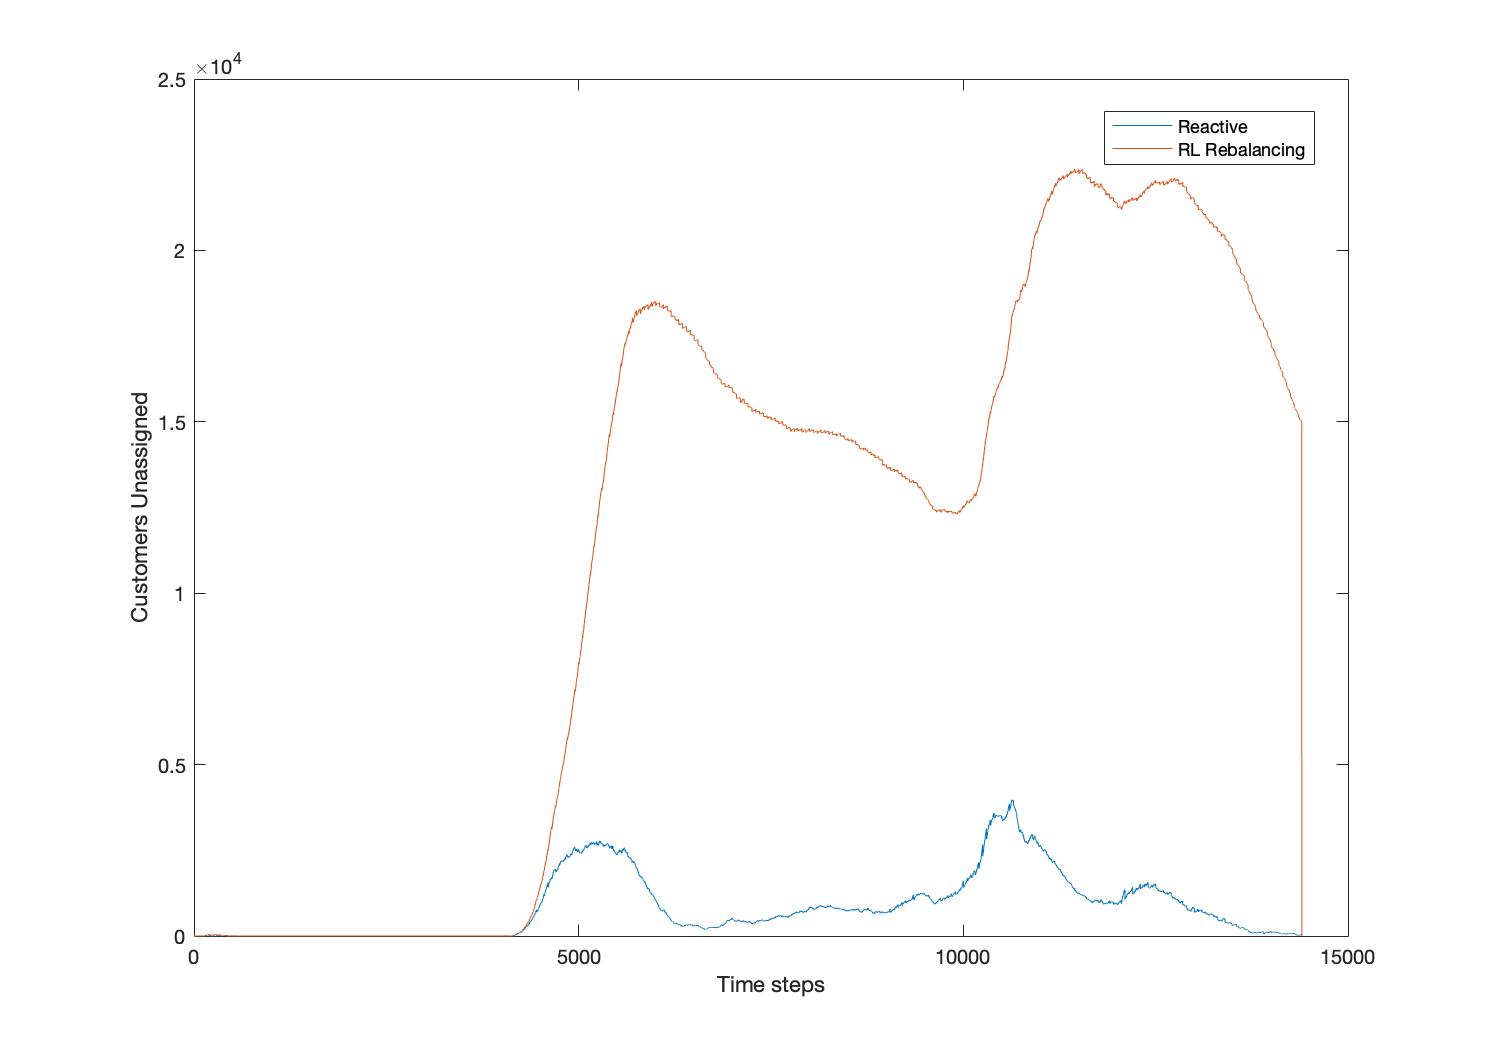
\includegraphics[scale=0.18]{custUnassigned.jpg}
      \caption{Number of customers unassigned}
      \label{figurelabel}
\end{figure}
\begin{figure}[thpb]
      \centering
      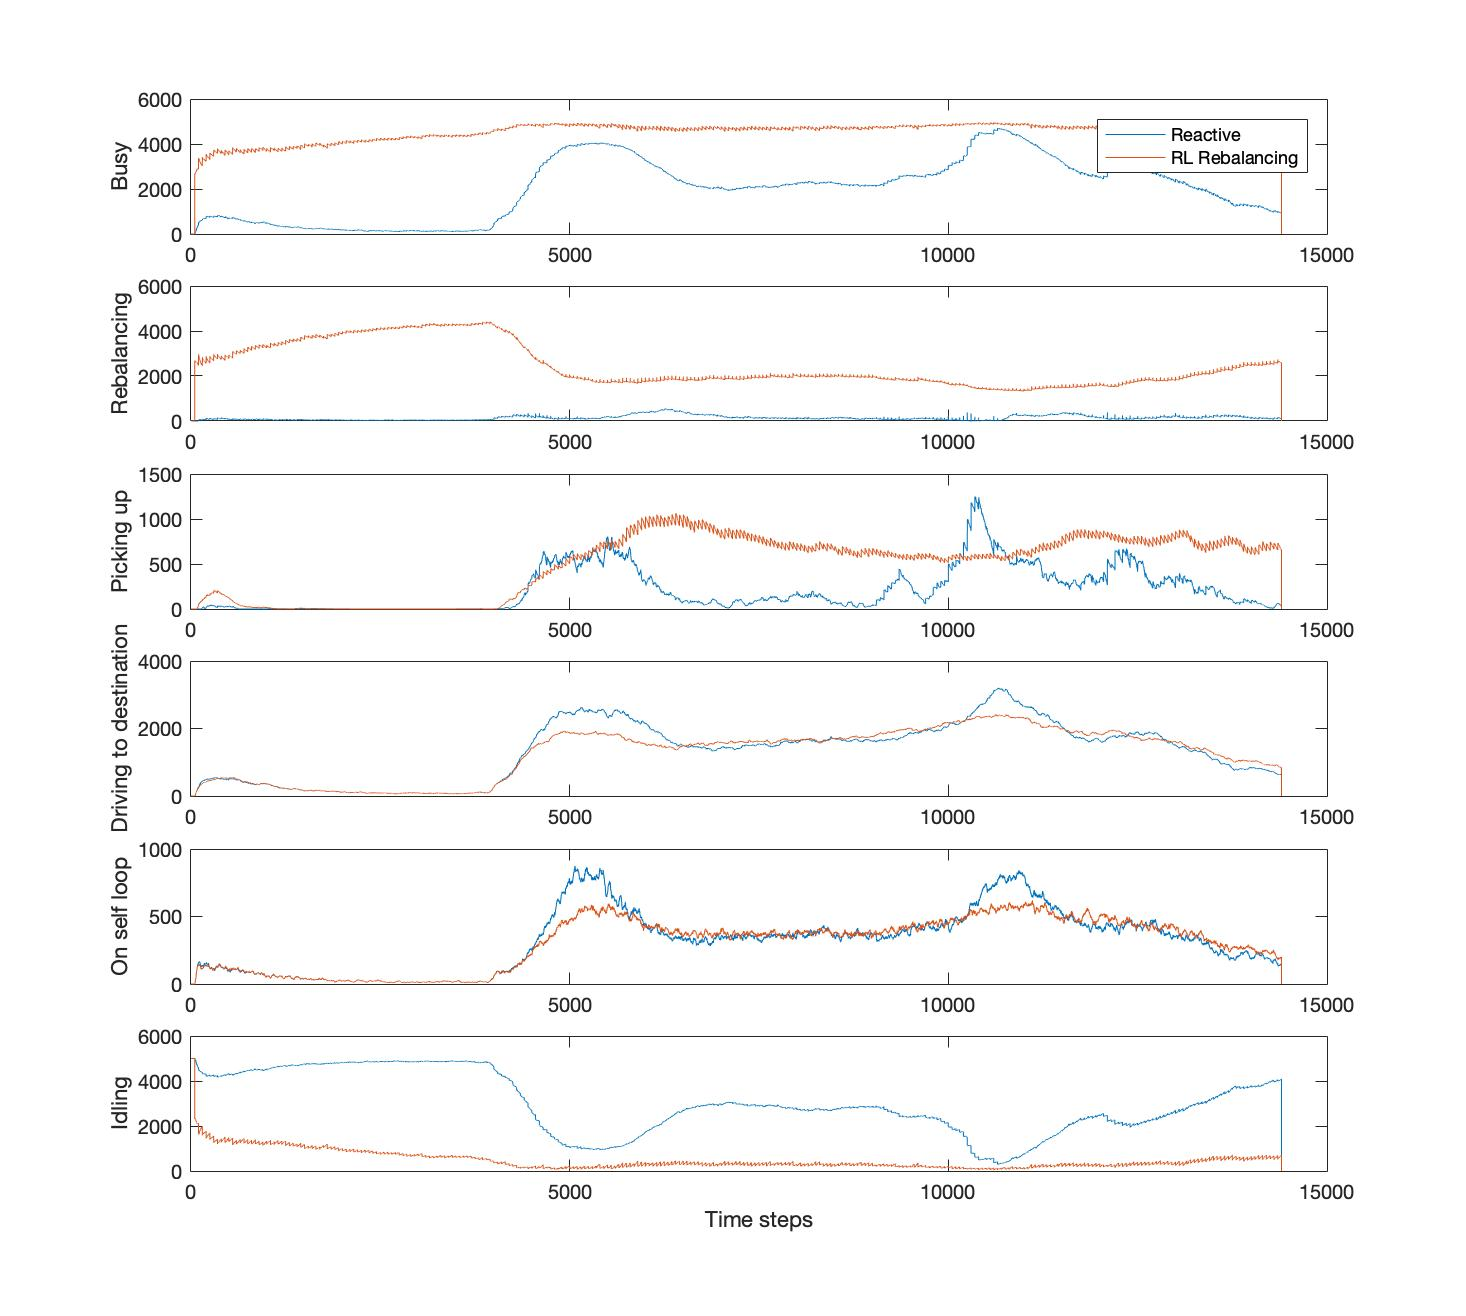
\includegraphics[scale=0.18]{vehicles.jpg}
      \caption{Vehicle behaviors}
      \label{figurelabel}
\end{figure}

Fig. 2 shows that in RL Rebalancing, a large number of customers are left unassigned. Taking a closer look at the vehicles' behaviors in Fig. 3, we can see that the number of vehicles rebalancing hugely exceeds that in Reactive, while the number of vehicles idling stays low. This means that most vehicles chose the actions of rebalancing, but to places that are not as demanding, therefore not causing them to pick up customers. 

\addtolength{\textheight}{-3cm}   % This command serves to balance the column lengths
                                  % on the last page of the document manually. It shortens
                                  % the textheight of the last page by a suitable amount.
                                  % This command does not take effect until the next page
                                  % so it should come on the page before the last. Make
                                  % sure that you do not shorten the textheight too much.

%%%%%%%%%%%%%%%%%%%%%%%%%%%%%%%%%%%%%%%%%%%%%%%%%%%%%%%%%%%%%%%%%%%%%%%%%%%%%%%%
%%%%%%%%%%%%%%%%%%%%%%%%%%%%%%%%%%%%%%%%%%%%%%%%%%%%%%%%%%%%%%%%%%%%%%%%%%%%%%%%
\section{Conclusions}
\subsection{Conclusions}
In this paper, we presented a reinforcement learning approach to rebalance vehicles. We first learn to approximate state-action values with historical data, then leverage the approximation to compute values associated with each action under a certain state, thereby being able to take actions corresponding to high values. Experiments based on real-world data show that this approach in application suffer from a great loss in performance, but does provide a solution that is more scalable than other alternatives reviewed. 

\subsection{Future Work}
As seen in the experiments section, althought theoretically this approach should achieve a good performance given that values are approximated correctly, it is not performing up to standards. More work will need to be done in adjusting state and reward definitions, other tunable parameters, in order to improve performance. 

On the other hand, we could explore whether performance could be improved if taking actions sequentially, therefore maximizing the amount of information each agent can obtain by knowing other agents' actions before it, which could improve the performance of this approach. A proposed algorithm for sequential learning and rebalancing process could be found in the appendix. 

Other future work include addressing the limitations in large state-space. VFA may not be a good approximation since the relationship between $x_t$, the weights $\textbf{w}$ and $Q(s_t,a_t;\textbf{}w)$ may not be linear. Advanced deep learning techniques like deep Q network could be leveraged to approximate large state-space with non-linearity. 

\bibliographystyle{unsrt} 
\bibliography{Biblio}  

\section*{Appendix}
\subsection{Derivation of $\nabla_\textbf{w} J$}
For simplicity of notation, let $s = s_t$,$a = a_t$,$s' = s_{t+1}$,$a' = a_{t+1}$, where $a'$ is derived from a policy (e.g. epsilon-greedy). Let $x$ be the vector of $s$ concatenated with a bias term, and $x'$ be that of $s'$.
In algorithm (1), we saw that
\begin{align*}
    J &= (Q_{target}-Q_{prediction})^2\\
    &= [Q(s,a;\textbf{w})-(r+\gamma Q(s',a'))]^2
\end{align*}
Since $Q(s,a;\textbf{w})=(\textbf{w}x)_a$,
\begin{align*}
    J &= (\textbf{w}x)_a-r-\gamma(\textbf{w}x)_a\\
    &= (\textbf{w}_{a,:} x - r - \gamma \textbf{w}_{a',:}x')^2\\
    \nabla_\textbf{w}J &= 2(\textbf{w}_{a,:} x - r - \gamma \textbf{w}_{a',:}x')\cdot
    \begin{cases}
      x^T, & \text{if}\ a^{th} row \\
      -\gamma x'^T, & \text{if}\ a'^{th} row\\
      0, & \text{otherwise}
    \end{cases}
\end{align*}
\subsection{Algorithms for learning and rebalancing sequentially}
\begin{algorithm}[H]
\caption{Learning Stage: SARSA with VFA, Sequential}
\begin{algorithmic}
\For{each time step $t \in {0,1,...,T}$ }
    \State Observe $\hat{s}_t=s_t$
    \For{each vehicle $m$}
        \If {vehicle is idle}
            \State $a^m_t \leftarrow \pi(s_t)$ 
            \State $\hat{s}_t \leftarrow$ \textbf{simulate} $(a^m_t,s_t)$
        \EndIf
        \State Observe $r_{t-1}$
        \State $\textbf{w} \leftarrow \textbf{w} - \alpha \nabla_{ \textbf{w}} J$
    \EndFor
    \State\textbf{Assign} $\{a^1_t,a^2_t,...,a^M_t\}$
\EndFor
\end{algorithmic}
\end{algorithm}
\begin{algorithm}[H]
\caption{Rebalancing Stage: Sequentially Performing Actions}
\begin{algorithmic}
\For{each time step $t \in {0,1,...,T}$}
    \State Observe $\hat{s}_t=s_t$
    \For{each vehicle $m$}
        \If {vehicle is idle}
            \State $a_t^m \leftarrow \argmax_a(Q(\hat{s}_t,a))$
            \State $\hat{s}_t \leftarrow$ \textbf{simulate}$(a^m_t,s_t)$
        \EndIf
    \EndFor
    \State\textbf{Assign}$\{a^1_t,a^2_t,...,a^M_t\}$
\EndFor
\end{algorithmic}
\end{algorithm}
We create smaller simulated states, $\hat{s_t}$ that are updated every time a vehicle has been assigned an action. By doing this, we should theoretically be able to find the global optimum by assigning actions sequentially for each vehicle. 



   




\end{document}
